\subsection{Parallel Simulation}
We now continue by describing our parallel simulation performance for different synchronization protocols, and compared to \textit{adevs}.
The speedup of \textit{adevs} is computed with the corresponding \textit{dxex} sequential benchmark.
This was done to take into account the performance difference observed in sequential simulation.

\subsubsection{Queue}
The Queue model is one single chain of models, resembling a pipeline.
This structure can be exploited to prevent cyclic dependencies in the parallel simulation.

Figure~\ref{fig:Queue_plot_strong} shows the speedup compared to sequential simulation for a fixed problem size.
%TODO this is actually quite a strange choice...
As the number of kernels increases, the optimistic kernel quickly becomes the worst choice.
This is mainly caused by the pipeline structure of the model: the last models in the queue only respond to incoming messages and therefore have to be rolled back frequently.
The difference between \textit{dxex} conservative and \textit{adevs} becoms smaller when more and more cores are used.
The same effect can be seen for weak scaling in Figure~\ref{fig:Queue_plot_weak}.

\begin{figure}
	\center
	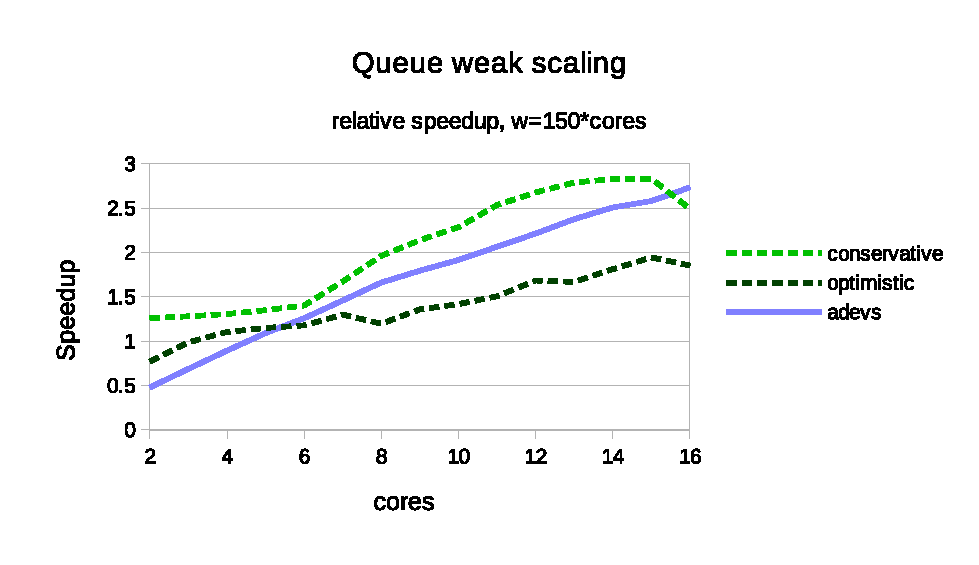
\includegraphics[width=\columnwidth]{fig/queue_fixed_weak_speedup.eps}
	\caption{Queue model weak scaling speedup compared to \textit{dxex} sequential.}
	\label{fig:Queue_plot_weak}
\end{figure}
	
\begin{figure}
	\center
	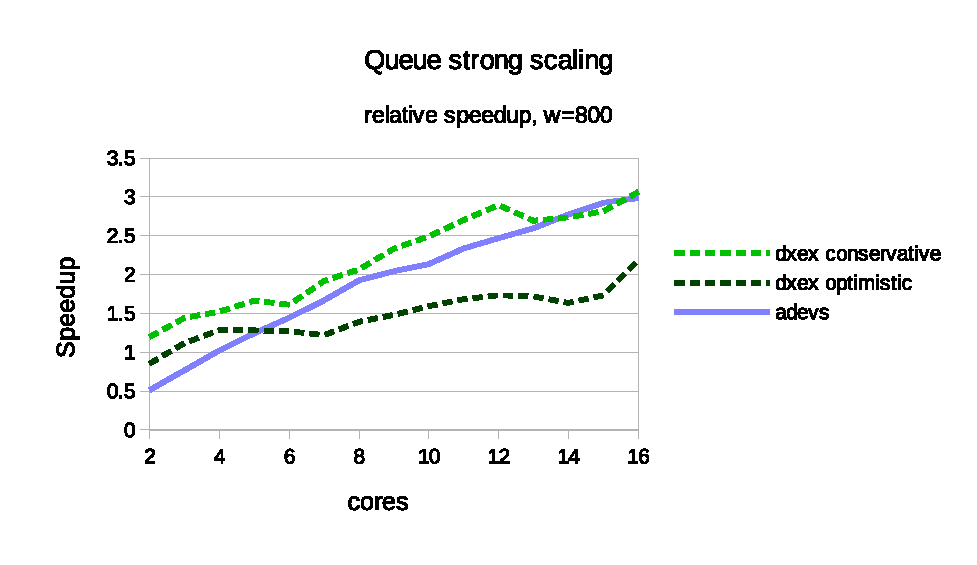
\includegraphics[width=\columnwidth]{fig/queue_fixed_strong_speedup.eps}
	\caption{Queue model strong scaling speedup compared to \textit{dxex} sequential.}
	\label{fig:Queue_plot_strong}
\end{figure}

\subsubsection{Interconnect}\label{subsec:parallelinterconnect}
In the Interconnect model, we determine how broadcast communication is supported across multiple nodes.
The number of models is now kept constant at eight.
Results are shown in Figure~\ref{fig:interconnect_benchmark_parallel}.
When the number of nodes increases, performance decreases due to increasing contention in conservative simulation and the increasing number of rollbacks in optimistic simulation.
All models depend on each other and have no computational load whatsoever, negating any possible performance gain by executing the simulation in parallel.

\begin{figure}
	\center
	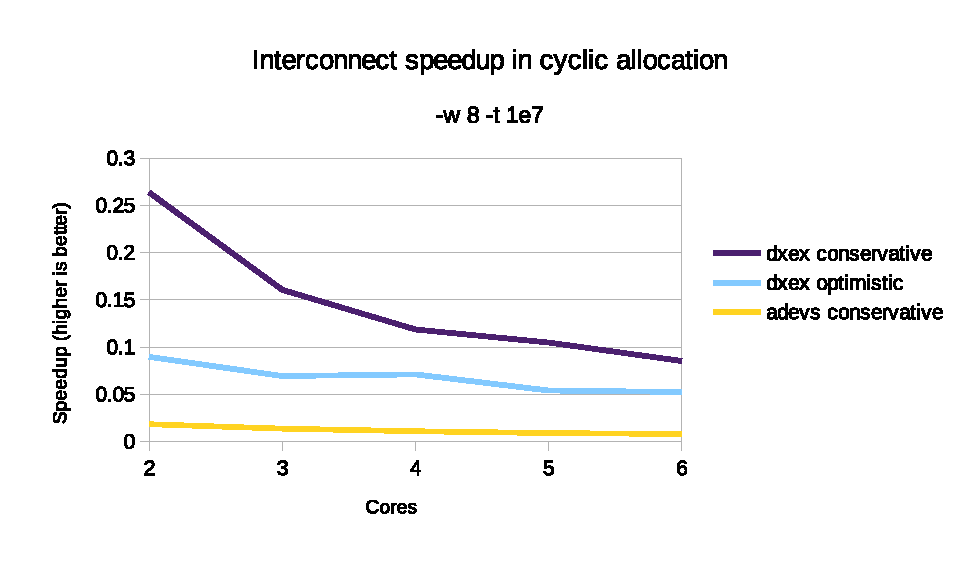
\includegraphics[width=\columnwidth]{fig/interconnect_parallel.eps}
	\caption{Interconnect benchmark results for parallel simulation.}
	\label{fig:interconnect_benchmark_parallel}
\end{figure}

\subsubsection{PHOLD}
In the PHOLD model, we first investigate the influence of the percentage of remote events on the speedup.
A remote event in this context is an event that is sent from a model on one kernel to a model on another simulation kernel.
When remote events are rare, optimistic synchronization rarely has to roll back, thus increasing performance.
With more common remote events, however, optimistic synchronization quickly slows down due to frequent rollbacks.
Conservative synchronization, on the other hand, is mostly unconcerned with the number of remote events: the mere fact that a remote event can happen, causes it to block and wait.
Even though a single synchronization protocol is always ideal in this case, it already shows that different synchronization protocols respond differently to a changing model.

\textit{Adevs} is significantly slower during conservative synchronization.
Analysis of profiling callgraphs shows that exception handling in \textit{adevs} is the main cause. 
To keep the models equivalent, the \textit{adevs} version does not provide the \{begin,end\}Lookahead methods, which accounts for the exception handling.
These functions require the user to implement a state saving method.
But in contrast to \textit{PythonPDEVS} and \textit{dxex}, which handle this inside the kernel, users need to manually define this.
We feel this would lead to an unfair comparison as we would like to keep the models agnostic of the underlying protocols across all benchmarks.

\begin{figure}
    \center
    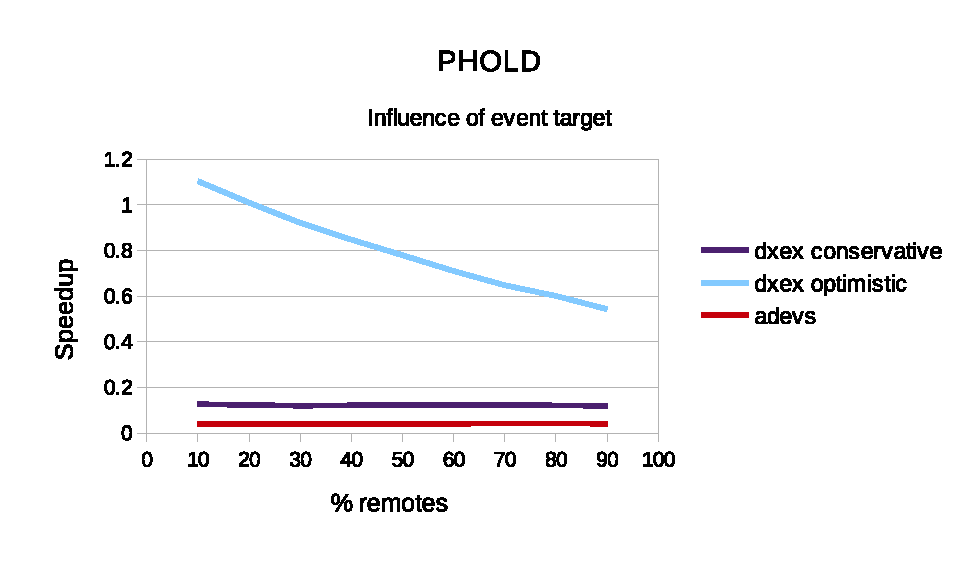
\includegraphics[width=\columnwidth]{fig/phold_remotes.eps}
    \caption{PHOLD benchmark results for parallel simulation using four kernels, four atomics per node, with varying percentage of remote events.}
\end{figure}
\begin{figure}
	\center
	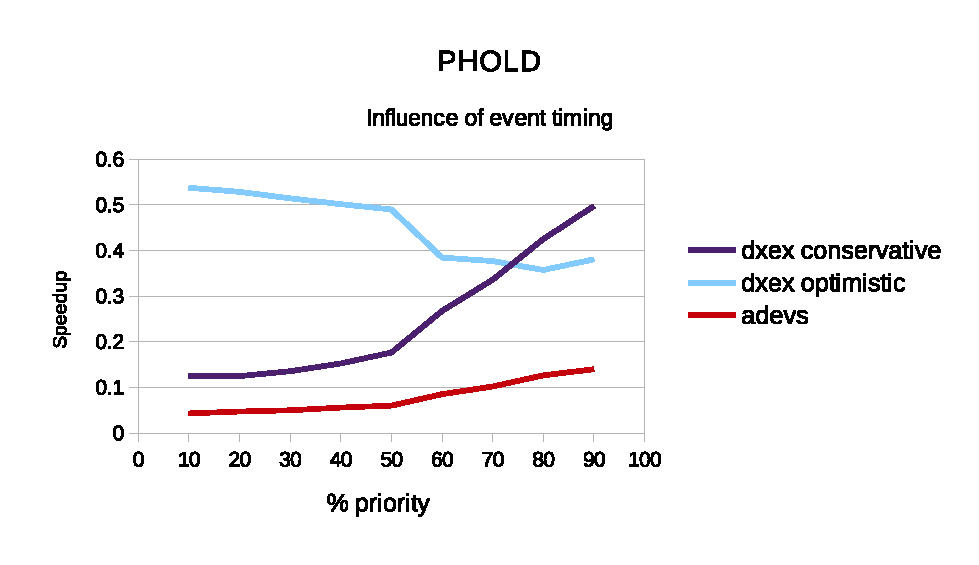
\includegraphics[width=\columnwidth]{fig/phold_priority.eps}
	\caption{PHOLD benchmark results for parallel simulation using four kernels, with varying amount of high-priority events.}
	\label{fig:phold_priority}
\end{figure}

We slightly modified the PHOLD benchmark to include high-priority events.
Contrary to normal events, high-priority events happen almost instantaneously, restricting lookahead to a very small value.
Even when normal events occur most often, conservative synchronization always blocks until it can make guarantees.
Optimistic synchronization, however, simply goes forward in simulation time and rolls back when these high-priority events happen.
This situation closely mimics the model typically used for comparing conservative and optimistic synchronization~\cite{FujimotoBook}.

Figure~\ref{fig:phold_priority} shows how simulation performance is influenced by the fraction of these high-priority events.
If barely any high-priority events occur, conservative synchronization is penalized due to its excessive blocking, which often turned out to be unnecessary.
When many high-priority events occur, optimistic synchronization is penalized due to its unconditional progression of simulation, which frequently needs to be rolled back.
Results show that there is no single perfect synchronization algorithm for this model: depending on configuration, either synchronization protocol might be better.
